\documentclass{beamer}
\usepackage[utf8]{inputenc}
\usepackage[english]{babel}
\usepackage{geometry}
\usepackage{amssymb}
\usepackage{amsfonts}
\usepackage{dsfont}
\usepackage{float}
\usepackage{graphicx}
\usepackage{wrapfig}
\usepackage{mathtools}
\usepackage{bbm}
\usepackage{amsthm}
\usepackage{ifthen}
\usepackage{graphicx}
\usepackage{hyperref}
\usepackage{tcolorbox}
\usepackage[ruled,vlined]{algorithm2e}
\usepackage{tikz}

\usepackage{caption}
\usepackage{subcaption}

%%%%%%%% box %%%%%%%%
\definecolor{mycolor}{rgb}{0.122, 0.435, 0.698}% Rule colour
\makeatletter
\newcommand{\mybox}[1]{%
	\setbox0=\hbox{#1}%
	\setlength{\@tempdima}{\dimexpr\wd0+13pt}%
	\begin{tcolorbox}[colframe=blue,boxrule=0.5pt,arc=4pt,
		left=6pt,right=6pt,top=6pt,bottom=6pt,boxsep=0pt,width=\@tempdima]
		#1
	\end{tcolorbox}
}
%%%%%%%%





\DeclarePairedDelimiter{\ceil}{\lceil}{\rceil}

\newcommand{\ca}[1]{\mathcal{#1}}
\newcommand{\bb}[1]{\mathbb{#1}}
\newcommand{\p}{\mathbb{P}}
\newcommand{\evento}[1]{\left\{ \textit{``#1''} \right\}}
\newcommand{\comillas}[1]{``#1''}
\newcommand{\set}[1]{\left\{#1\right\}}
\newcommand{\parent}[1]{\left(#1\right)}
\newcommand{\parentCuad}[1]{\left[#1\right]}
\newcommand{\borel}{\ca{B}(\bb{R}^d)}
\newcommand{\Rd}{\bb{R}^d}
\newcommand{\R}{\bb{R}}
\newcommand{\infNorm}[1]{||#1||_\infty}
\newcommand{\condExp}[2]{\bb{E}(#1|#2)}
\newcommand{\ind}[1]{\mathbbm{1}_{#1}}
\newcommand{\esp}[1]{\bb{E}\barras{#1}}
\newcommand{\indep}{\rotatebox[origin=c]{90}{$\models$}}
\newcommand{\pe}{$(\Omega, \ca{F}, \p)\ $}
\newcommand{\vc}[1]{\langle #1 \rangle}
\newcommand{\gb}[1]{\overline{\widehat{#1}}}
\newcommand{\barras}[1]{\left| #1 \right|}
\newcommand{\integral}{\int_{t_i}^{t_{i+1}}}
\newcommand{\ug}[1]{\widehat{\ca{U}}_{#1}}
\newcommand{\vg}[1]{\widehat{\ca{V}}_{#1}}
\newcommand{\zg}[1]{\widehat{\ca{Z}}_{#1}}
\newcommand{\norm}[1]{\left\lVert#1\right\rVert}
\newcommand{\X}{\ca{X}}
\newcommand{\xscheme}[1]{X_{t_{#1}}^{\pi}}
\newcommand{\prom}[1]{\langle #1 \rangle}


%\usetheme{Darmstadt default}
\usetheme{Copenhagen}
%\usetheme{Madrid}
%\usecolortheme{beaver}
\usecolortheme{seahorse}
\usefonttheme[onlymath]{serif}
\usefonttheme{structuresmallcapsserif}

\title[Análisis de Datos: Twitter]{Análisis de Datos: Twitter}
\author{Javier Castro M.}
\institute{Universidad De Chile}
\date{\today}

%exponer sus objetivos, descripción de la base de datos y de los métodos a aplicar


\begin{document}
	
	\maketitle
	
	\begin{frame}{Objetivos}
		\textbf{Motivación}: El principio del proyecto es entender cómo los datos impactan en el resultado de nuestro modelo. O bien, entender que los posibles sesgos que presenten nuestros datos se traspasaran a los resultados.
	\end{frame}

	\begin{frame}{Twint: \textbf{Tw}itter \textbf{In}telligence \textbf{T}ool}
		Desde el \textbf{github} de \textbf{twint}: \\
		\vspace{1cm}
		\comillas{Twint is an advanced Twitter scraping tool written in Python that allows for scraping Tweets from Twitter profiles without using Twitter's API.}
	\end{frame}

	\begin{frame}{Twitter en el estallido social}
		\begin{figure}[h]
			\centering
			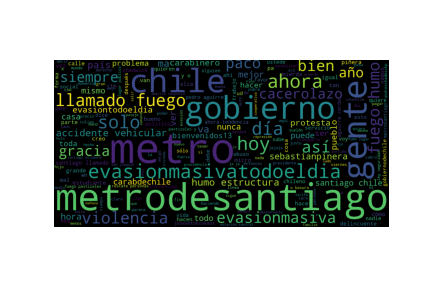
\includegraphics[scale=.5]{../imgs/wordcloud_santiago_estallido1.png}
			\caption{Wordcloud de twitter el $18$ de octubre del $2019$ con coordenadas en Beaucheff y un radio de $10km$.}
		\end{figure}
	\end{frame}

	\begin{frame}{Twitter en el día de la mujer}
		\begin{figure}[h]
			\centering
			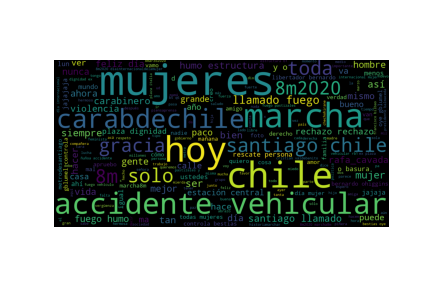
\includegraphics[scale=.5]{../imgs/wordcloud_santiago_8M.png}
			\caption{Wordcloud de twitter el $8$ de marzo del $2020$ con coordenadas en Beaucheff y un radio de $10km$.}
		\end{figure}
	\end{frame}

	\begin{frame}{Twitter en las votaciones pasadas}
		\begin{figure}[h]
			\centering
			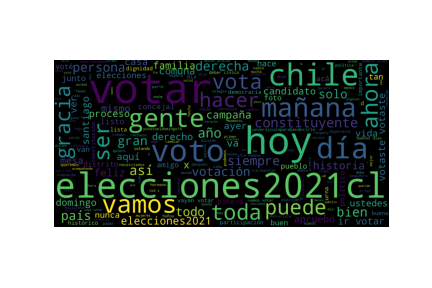
\includegraphics[scale=.5]{../imgs/wordcloud_chile_votaciones.png}
			\caption{Wordcloud de twitter durante las votaciones del $15$ y $16$ de mayo del $2021$ usando \texttt{.Near = "Santiago, Chile"}.}
		\end{figure}
	\end{frame}

	\begin{frame}{Fin}
		\centering
		\mybox{Muchas Gracias!}
	\end{frame}

	
	
	
\end{document}